\documentclass[sn-basic]{sn-jnl}

\usepackage{graphicx}
\usepackage{manyfoot}
\usepackage{textcomp}
\usepackage{amsmath,amssymb}
\usepackage{booktabs}
\usepackage{xcolor}
\usepackage{xurl}
\graphicspath{{figures/}}
\newcommand{\USD}{US\$}
\newcommand{\INR}{INR~}

\raggedbottom

\begin{document}

\title[M\&A and Financial Performance in the Gaming Industry]{A Case Study of the Impact of Mergers and Acquisitions on the Financial Performance of Companies in the Gaming Industry}

\author*[1]{\fnm{Harsh} \sur{Raj}}\email{applications.harsh@gmail.com}

\affil*[1]{\orgdiv{Department of Finance and Risk Engineering}, \orgname{New York University Tandon School of Engineering}, \orgaddress{\city{Brooklyn}, \state{NY}, \country{USA}}}

\abstract{\textbf{Purpose:} Video-game publishers have spent heavily on acquisitions since 2020, largely to buy into mobile gaming. This study asks whether those acquisitions improved the acquirers' financial performance.
\textbf{Methods:} Four cases are examined: Take-Two Interactive's \USD 12.7 billion purchase of Zynga, Electronic Arts' \USD 5.0 billion of acquisitions in 2021, Unity Software's \USD 4.4 billion merger with ironSource, and Nazara Technologies' acquisitions in India. Following Healy, Palepu and Ruback (1992), profitability, returns, cash flow and liquidity ratios from the acquirers' reported financial statements are compared for the three fiscal years before and after each deal, leaving out the year of completion.
\textbf{Results:} All four acquirers grew revenue, by 8.6\% to 42.1\% a year between the two windows, but three of the four became less profitable. Take-Two's operating margin fell from 15.3\% to $-48.9\%$ ($-13.3\%$ before \USD 5.9 billion of goodwill impairments), Electronic Arts' by 2.1 points and Nazara's by 12.6 points. Unity, loss-making before and after, was the only acquirer whose margins and cash flow improved. Goodwill rose to 20--46\% of the three US acquirers' assets, and the two acquirers whose announcement-day reaction could be measured lost 13\% of their market value that day.
\textbf{Conclusion:} In these cases, acquisitions bought revenue growth but not higher profitability; the market's scepticism at announcement proved largely justified.}

\keywords{Mergers and acquisitions, Post-merger performance, Video-game industry, Goodwill impairment, Mobile gaming, Case study}

\pacs[JEL Classification]{G34, L82, M41, L25}

\maketitle

\section{Introduction}\label{sec:intro}

Mergers and acquisitions (M\&A) are among the most important decisions a company makes. By buying another company, a firm can grow faster than it could by building, gain technology, talent and customers, and remove a competitor. Yet decades of research find that acquirers' shareholders gain little on average, and that many deals destroy value \citep{andrade2001,moeller2005}.

The video-game industry offers a clear recent test. Between 2020 and 2023 the largest publishers made a series of large acquisitions, most of them to build a position in mobile games, the industry's fastest-growing segment. Electronic Arts bought Codemasters, Glu Mobile and Playdemic in the first half of 2021; Take-Two Interactive bought Zynga, the maker of FarmVille and Words With Friends, for \USD 12.7 billion in 2022; Unity Software, the game-engine maker, merged with the mobile advertising company ironSource; and in India, Nazara Technologies built itself through a sequence of acquisitions. Microsoft's \USD 69 billion purchase of Activision Blizzard, completed in October 2023, is the largest deal in the industry's history, but gaming is too small a part of Microsoft for its effect to be seen in company-level figures, so it is not studied here.

This paper asks a simple question: did these acquisitions improve the acquirers' financial performance? It compares each acquirer's profitability, returns, cash flow and liquidity in the three fiscal years before and after its deal, using figures from its own financial statements. It contributes evidence from an industry that has received little attention in the post-merger performance literature, and documents the size of the goodwill write-downs that followed the largest deal.

\section{Literature review}\label{sec:lit}

Two approaches dominate research on whether acquisitions create value. Event studies measure the share-price reaction when a deal is announced. They find that target shareholders gain substantially, while acquirers' returns are close to zero on average and negative for large deals: \citet{moeller2005} found that acquiring-firm shareholders lost about \USD 240 billion in the merger wave of 1998--2001, concentrated in a small number of very large deals. \citet{roll1986} explained such losses by managerial hubris, in which acquirers overestimate the synergies they can capture and overpay.

The second approach, used in this paper, compares operating performance before and after the deal. \citet{healy1992} studied the 50 largest US mergers of 1979--1984 and found that merged firms' operating cash flow returns on assets improved relative to their industries, driven by better asset productivity rather than cost cuts. Later studies are less favourable. \citet{andrade2001} summarise the evidence as showing modest operating improvements at best. \citet{lubatkin1983} argued that the benefits of mergers are often offset by the costs of integrating two organisations, and \citet{epstein2005} identified strategic fit, deal structure and integration as the main determinants of merger success. \citet{gu2011} showed that acquirers with overpriced shares tend to overpay, and that the overpayment later appears as goodwill impairment.

Studies of India, where M\&A activity grew after liberalisation, find mixed results. \citet{vanitha2007} compared the financial performance of Indian manufacturing companies before and after merger; \citet{mantravadi2008} found that effects differ by industry, with improvements in some sectors and declines in others; and \citet{pazarskis2006} found deterioration after mergers in Greece.

Few of these studies cover the video-game industry, whose assets are largely intangible (intellectual property, studios and players) and whose revenues depend on a small number of hit titles. These features make acquisitions both attractive, as a way to buy proven franchises and players, and risky, because the purchased assets can lose value quickly.

\section{Data and methods}\label{sec:methods}

\subsection{Cases}

Table~\ref{tab:deals} lists the four cases. They were chosen because each acquirer is a listed games company for which the deal was material, and for which at least three fiscal years of reported figures are available before and after completion. Electronic Arts completed three acquisitions within five months (Codemasters in February 2021, Glu Mobile in April 2021 and Playdemic in June 2021), which are treated as one event. Nazara Technologies bought controlling stakes in Sportskeeda and Paper Boat Apps (Kiddopia) in 2019 and has continued acquiring since, most recently PokerBaazi's parent Moonshine Technology (\INR 9.82 billion for 47.7\%, 2024) and Curve Games (\INR 2.47 billion, 2025) \citep{bs2024nazara,bs2025nazara}.

\begin{table}[h]
\caption{The four acquisitions}\label{tab:deals}
\footnotesize
\setlength{\tabcolsep}{4pt}
\begin{tabular}{@{}p{2.2cm}p{2.5cm}rp{3.8cm}l@{}}
\toprule
Acquirer & Target & Value & Payment & Completed \\
\midrule
Take-Two Interactive & Zynga & \USD 12.7 bn & \USD 3.50 cash plus 0.0406 Take-Two shares per Zynga share & May 2022 \\
Electronic Arts & Codemasters, Glu Mobile, Playdemic & \USD 5.0 bn & Cash (\USD 1.2, 2.4 and 1.4 bn) & Feb--Jun 2021 \\
Unity Software & ironSource & \USD 4.4 bn & All stock, 0.1089 Unity shares per ironSource share & Nov 2022 \\
Nazara Technologies & Sportskeeda (67\%), Paper Boat Apps (51\%) & \INR 1.28 bn & Cash (\INR 0.44 and 0.84 bn) & 2019 \\
\botrule
\end{tabular}
\footnotetext{Sources: \citet{bwzynga}, \citet{wikiea}, \citet{eaglu}, \citet{tc2022unity}, \citet{wikinazara}.}
\end{table}

\subsection{Data}

Annual figures for Take-Two, Electronic Arts and Unity (revenue, operating income, net income, total assets, shareholders' equity, current assets and liabilities, operating cash flow, goodwill and goodwill impairment) were taken from their annual reports on Form 10-K through the XBRL data published by the US Securities and Exchange Commission \citep{secttwo,secea,secunity}, using the most recently reported figure for each year. Nazara's consolidated figures were taken from Screener.in \citep{screener}; its operating profit is reported before depreciation, interest and tax, and its current assets, current liabilities and goodwill are not available. All figures are published with this paper.

\subsection{Measures and design}

For each acquirer and fiscal year $t$, the following ratios are computed:
\begin{align}
\text{Operating margin}_t &= \frac{\text{Operating income}_t}{\text{Revenue}_t}, &
\text{ROA}_t &= \frac{\text{Net income}_t}{\text{Total assets}_t}, \nonumber\\
\text{ROE}_t &= \frac{\text{Net income}_t}{\text{Equity}_t}, &
\text{OCF/A}_t &= \frac{\text{Operating cash flow}_t}{\text{Total assets}_t}, \nonumber\\
\text{Current ratio}_t &= \frac{\text{Current assets}_t}{\text{Current liabilities}_t}, &
\text{GW/A}_t &= \frac{\text{Goodwill}_t}{\text{Total assets}_t}. \label{eq:ratios}
\end{align}
Because goodwill impairments are non-cash charges that reflect a revaluation of past purchases rather than current operations, operating margin is also reported with the impairment added back. The operating cash flow return on assets follows \citet{healy1992}, who preferred cash flow because it is not affected by the accounting method used for the acquisition.

Year 0 is the fiscal year in which the deal completed (for Electronic Arts, the year in which most of the acquisitions completed). Following \citet{healy1992}, year 0 is left out because it combines pre- and post-deal operations and carries one-off transaction costs. For each measure $x$, the change is
\begin{equation}
\Delta x = \frac{1}{3}\sum_{t=1}^{3} x_{t} - \frac{1}{3}\sum_{t=-3}^{-1} x_{t}.\label{eq:change}
\end{equation}
Revenue growth is measured as the compound annual growth rate between the average revenue of the two windows.

With four cases, no statistical test can establish an average effect: the smallest two-sided $p$-value attainable by a sign test or Wilcoxon signed-rank test on four observations is 0.125. The results are therefore presented as case evidence. Unlike \citet{healy1992}, the ratios are not adjusted for industry performance, so part of each change may reflect conditions common to the industry, notably the fall in games spending after the pandemic boom.

\section{Results}\label{sec:results}

\subsection{Revenue and profitability}

Table~\ref{tab:results} reports the before-and-after averages. All four acquirers grew revenue, from 8.6\% a year at Electronic Arts to 42.1\% at Nazara, largely because the acquired businesses' revenues were added to their own. Profitability moved the other way at three of the four (Figure~\ref{fig:margins}).

\begin{table}[t]
\caption{Financial performance in the three fiscal years before and after each deal}\label{tab:results}
\scriptsize
\setlength{\tabcolsep}{3pt}
\begin{tabular}{@{}lrrrrrrrr@{}}
\toprule
 & \multicolumn{2}{c}{Take-Two} & \multicolumn{2}{c}{Electronic Arts} & \multicolumn{2}{c}{Unity} & \multicolumn{2}{c}{Nazara} \\
 & Before & After & Before & After & Before & After & Before & After \\
\midrule
Revenue growth a year & \multicolumn{2}{c}{+15.3\%} & \multicolumn{2}{c}{+8.6\%} & \multicolumn{2}{c}{+24.6\%} & \multicolumn{2}{c}{+42.1\%} \\
Operating margin & 15.3\% & $-48.9$\% & 21.6\% & 19.5\% & $-37.1$\% & $-35.2$\% & 23.1\% & 10.6\% \\
\quad before impairments & 15.3\% & $-13.3$\% & 21.6\% & 19.5\% & $-37.1$\% & $-35.2$\% & 23.1\% & 10.6\% \\
Net margin & 14.2\% & $-51.3$\% & 30.1\% & 14.2\% & $-38.2$\% & $-32.0$\% & 12.3\% & 5.6\% \\
Return on assets & 8.1\% & $-27.5$\% & 15.0\% & 8.2\% & $-14.3$\% & $-9.0$\% & 8.2\% & 2.9\% \\
Return on equity & 14.9\% & $-94.7$\% & 23.5\% & 15.2\% & $-25.8$\% & $-19.7$\% & 9.8\% & 4.2\% \\
Cash flow / assets & 11.0\% & 2.0\% & 16.0\% & 15.2\% & $-3.5$\% & 4.7\% & 8.6\% & 3.9\% \\
Current ratio & 1.81 & 0.98 & 2.57 & 1.18 & 2.89 & 2.32 & -- & -- \\
Goodwill / assets & 9.0\% & 19.7\% & 19.9\% & 41.2\% & 24.3\% & 45.7\% & -- & -- \\
\botrule
\end{tabular}
\footnotetext{Averages of the three fiscal years before and after the deal, excluding the year of completion: Take-Two FY2020--22 and FY2024--26; Electronic Arts FY2019--21 and FY2023--25; Unity FY2019--21 and FY2023--25; Nazara FY2017--19 and FY2021--23. Cash flow is operating cash flow. Nazara's operating margin is before depreciation. Electronic Arts' net margin, ROA and ROE before the deals are raised by a one-off tax benefit in FY2020. Sources: \citet{secttwo,secea,secunity,screener}; author's calculations.}
\end{table}

\begin{figure}[t]
\centering
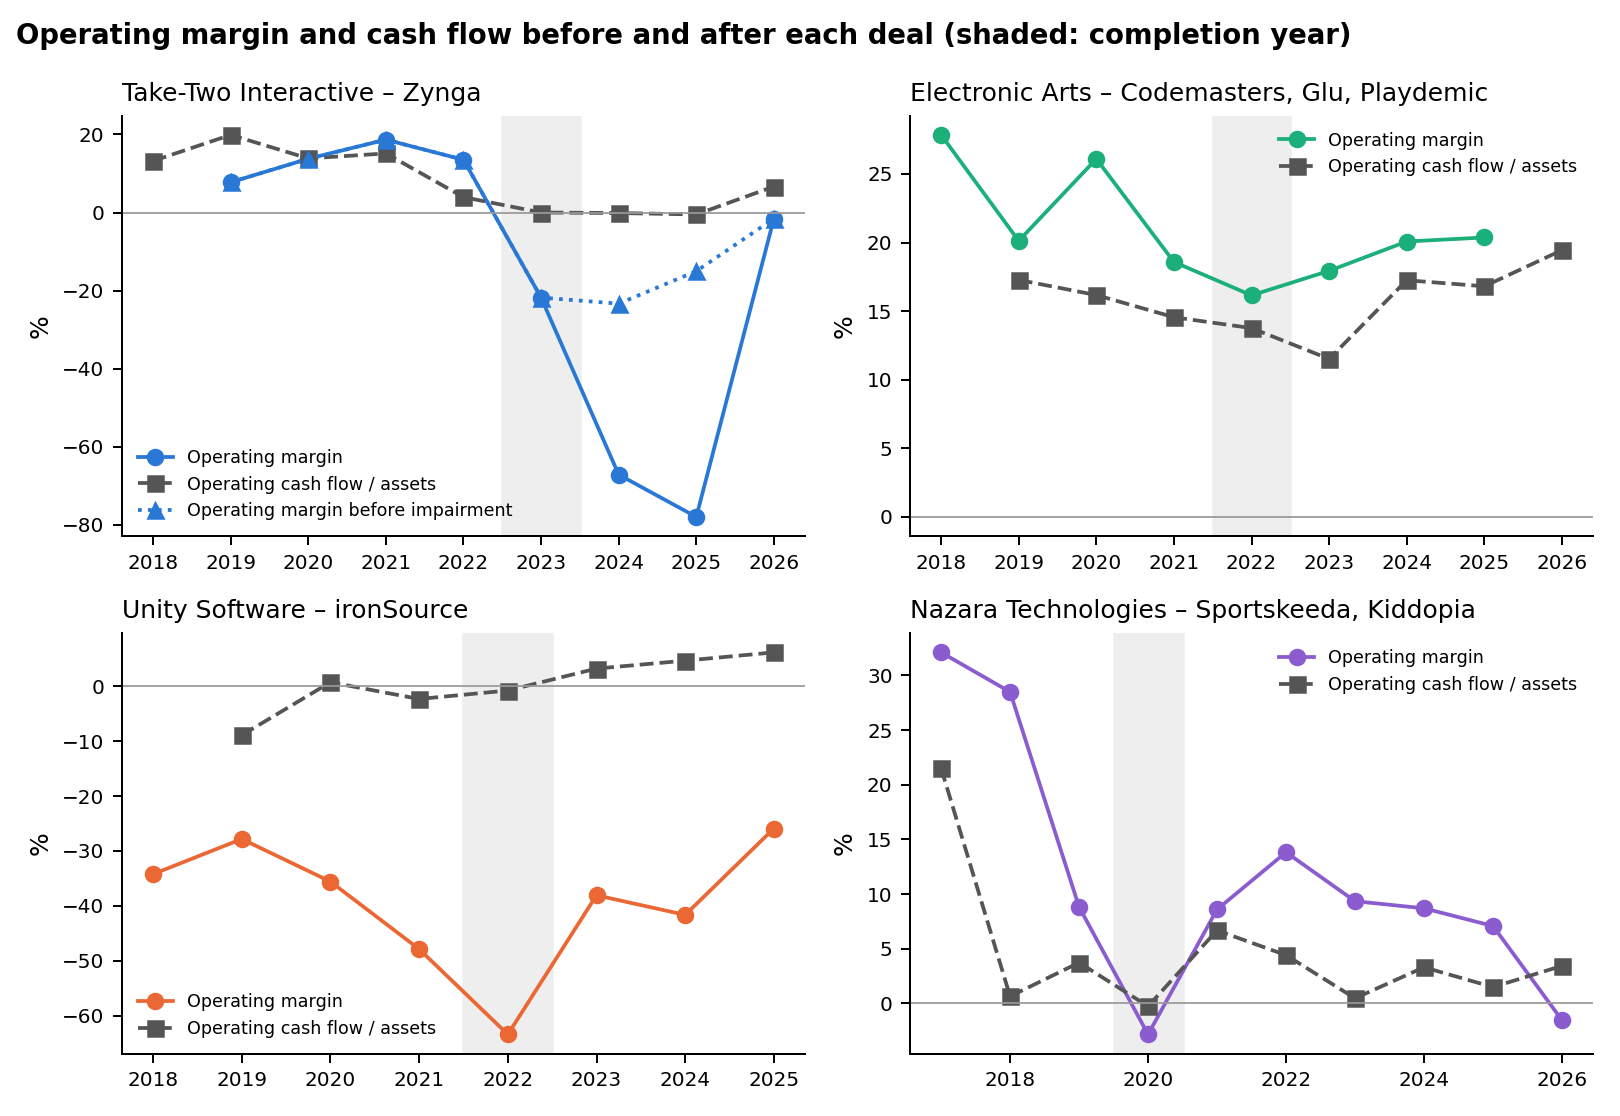
\includegraphics[width=\textwidth]{margins.png}
\caption{Operating margin and operating cash flow to assets by fiscal year; the shaded band marks the year each deal completed}\label{fig:margins}
\end{figure}

\textbf{Take-Two and Zynga.} Revenue averaged \USD 5.88 billion after the deal against \USD 3.32 billion before, but the operating margin fell from 15.3\% to $-48.9\%$. Two forces drove the fall. First, the amortisation of Zynga's acquired intangible assets turned an operating profit into a loss of \USD 1.17 billion in FY2023, the year of completion. Second, Take-Two wrote down \USD 2.34 billion of goodwill in FY2024 and \USD 3.55 billion in FY2025, \USD 5.89 billion in total, largely relating to the Zynga business. With the impairments added back, the operating margin still fell by 28.6 points, and operating cash flow, which had averaged 11.0\% of assets, was close to zero from FY2023 to FY2025 before recovering to \USD 624 million in FY2026. Goodwill, which had been 9--10\% of assets, jumped to 43\% after the deal and fell back to 11\% after the write-downs.

\textbf{Electronic Arts.} The three acquisitions added revenue and lifted growth to 8.6\% a year, while the operating margin slipped from 21.6\% to 19.5\% and the operating cash flow return was almost unchanged. Of the four cases, this is the closest to neutral. The fall in net margin and ROA overstates the deterioration, because EA's pre-deal net income includes a one-off tax benefit in FY2020. Paying \USD 5.0 billion in cash more than halved the current ratio, from 2.57 to 1.18, and goodwill doubled from about a fifth to over 40\% of assets, where it has stayed at about \USD 5.4 billion.

\textbf{Unity and ironSource.} Unity was loss-making before and after the merger. ironSource's advertising business raised revenue by 57\% in 2023 and turned operating cash flow positive, from $-3.5\%$ to 4.7\% of assets, but operating losses narrowed only from 37.1\% to 35.2\% of revenue. Revenue then fell 17\% in 2024. Goodwill rose to about 46\% of assets and has been unchanged since 2023.

\textbf{Nazara.} Revenue quadrupled, from an average of \INR 1.77 billion to \INR 7.22 billion, after the 2019 acquisitions and those that followed. The margin before depreciation fell from 23.1\% to 10.6\%, and returns on assets and equity roughly halved. Nazara has continued to acquire, and in FY2026 its operating result before depreciation turned negative for the first time since FY2020.

\subsection{Balance sheets and market reaction}

Figure~\ref{fig:goodwill} shows how the three US acquisitions transformed their buyers' balance sheets. Goodwill rose to 40--46\% of total assets at Electronic Arts and Unity and to 43\% at Take-Two, meaning that a large share of each company's assets consisted of the premium paid over the value of the businesses bought. At Take-Two most of that premium has since been written off.

\begin{figure}[h]
\centering
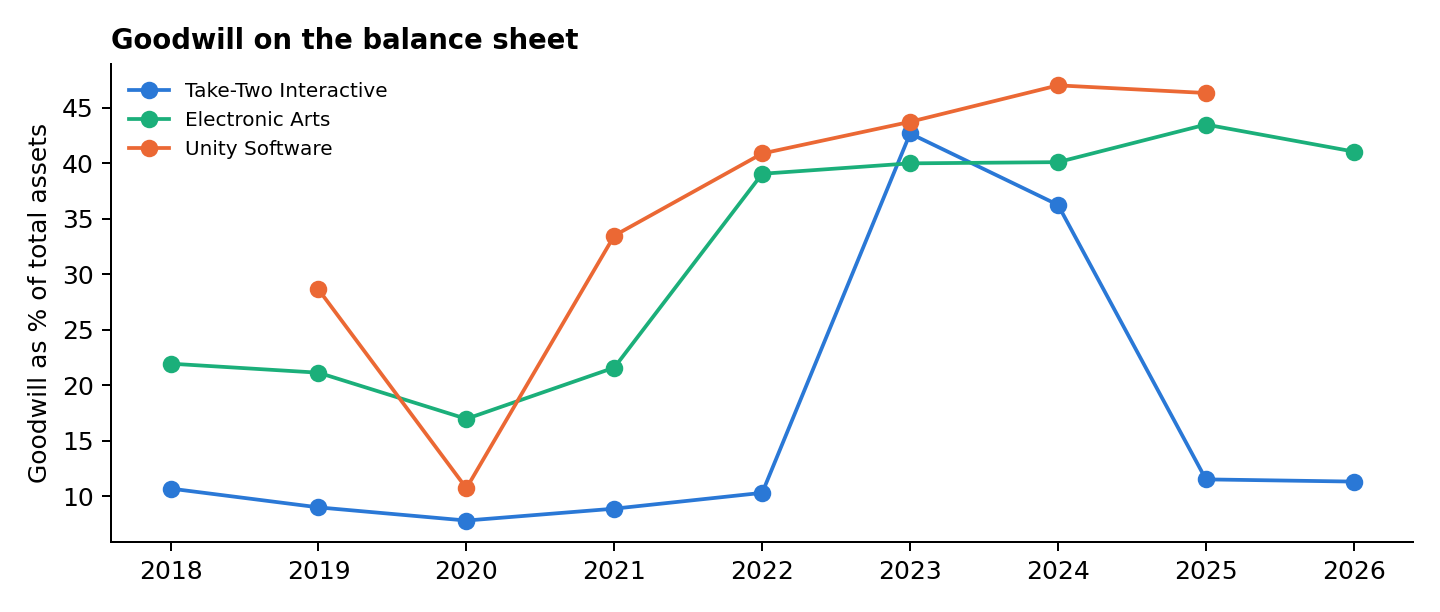
\includegraphics[width=0.9\textwidth]{goodwill.png}
\caption{Goodwill as a share of total assets, fiscal years 2018--2026}\label{fig:goodwill}
\end{figure}

The stock market anticipated these outcomes. Take-Two's shares fell 13.1\% on the day the Zynga deal was announced, their largest one-day fall since 2009, while Zynga's rose 40.7\% on a 64\% premium \citep{vgc2022}. Unity's shares fell about 13\% on the day it announced the ironSource merger \citep{cnbc2022unity}, although the same announcement cut its revenue guidance, so the fall cannot be attributed to the merger alone.

\section{Discussion}\label{sec:discussion}

The four cases fit the pattern in the wider literature more closely than the optimistic view in much practitioner writing. Every acquisition delivered its most visible promise, a larger and faster-growing business, but three of the four acquirers earned less on their revenue and assets afterwards. In the largest deal, the post-merger losses and \USD 5.9 billion of impairments are consistent with overpayment \citep{roll1986,gu2011}: Take-Two paid a 64\% premium for Zynga at the peak of pandemic-era demand for mobile games, and the value of the purchase fell once that demand normalised. Electronic Arts, which paid less relative to its own size and in cash, kept its margins close to their previous level.

Three lessons follow for managers and investors. First, revenue growth after an acquisition is largely mechanical and says little about whether the deal created value; profitability, cash flow and returns on the enlarged asset base are the relevant measures. Second, the price paid matters as much as strategic fit: a deal bought at the top of a cycle carries its premium on the balance sheet as goodwill, which is written off if the cycle turns. Third, the market's initial reaction deserves weight: in both cases where it could be measured, the acquirer's share price fell sharply on announcement, and the subsequent accounting results bore out that scepticism.

The study has important limitations. Four cases cannot establish an average effect, and the choice of cases reflects data availability. The ratios are not adjusted for industry conditions, so part of the decline reflects the fall in games spending after the pandemic, which affected acquirers and non-acquirers alike. Before-and-after comparisons cannot say what would have happened without the deal. The post-deal windows are short for Take-Two and Unity, whose integration continues. Nazara's figures come from a secondary source and exclude some balance-sheet items, and its later acquisitions overlap with the post-deal window.

Future work should extend the sample to all listed games acquirers since 2015, adjust performance against non-acquiring peers, and combine operating measures with long-run share-price returns.

\section{Conclusion}\label{sec:conclusion}

The original motivation for this study was the belief that mergers and acquisitions improve the financial performance of gaming companies. The evidence from four recent cases does not support that belief as a general rule. Acquisitions made the acquirers bigger: revenue grew at every one. But at three of the four, operating margins, returns on assets and cash flow were lower afterwards, and the largest deal was followed by nearly \USD 6 billion of goodwill write-downs. Only Unity, starting from deep losses, improved on these measures. In the gaming industry, as elsewhere, an acquisition's success depends less on the growth it buys than on the price paid for it.

\backmatter

\section*{Declarations}

\begin{itemize}
\item \textbf{Funding:} No funding was received for this study.
\item \textbf{Competing interests:} The author has no competing interests to declare.
\item \textbf{Ethics approval and consent to participate:} Not applicable; the study uses only published company data.
\item \textbf{Data availability:} All financial data and deal details used in this study are available at \url{https://github.com/harsh-github007/Gaming-MA-Financial-Performance}.
\item \textbf{Code availability:} The analysis script and figures are available in the same repository, and the results can be explored at \url{https://harsh-github007.github.io/Gaming-MA-Financial-Performance/}.
\item \textbf{Author contributions:} Harsh Raj designed the study, collected and analysed the data and wrote the manuscript.
\end{itemize}

\bibliography{references}

\end{document}
